\documentclass[10pt,a4paper]{article}
\usepackage[margin=2.2cm]{geometry}
\usepackage[T1]{fontenc}
\usepackage[utf8]{inputenc}
\usepackage{lmodern,microtype}
\usepackage{xcolor}
\usepackage{booktabs,tabularx,array,longtable}
\usepackage{amsmath,amssymb}
\usepackage{tikz}
\usetikzlibrary{arrows.meta,positioning,calc,fit,shapes.geometric}
\usepackage{hyperref}
\definecolor{navy}{HTML}{123047}
\definecolor{teal}{HTML}{007C7A}
\definecolor{sky}{HTML}{DCEFF1}
\definecolor{orange}{HTML}{E67E22}
\definecolor{pale}{HTML}{F4F6F7}
\hypersetup{colorlinks=true,linkcolor=navy,citecolor=navy,urlcolor=navy,pdftitle={Semi-Humanoid Robotics Software: Unified Literature Review}}
\setlength{\parindent}{1.1em}
\setlength{\parskip}{0.25em}
\renewcommand{\arraystretch}{1.15}
\newcolumntype{Y}{>{\raggedright\arraybackslash}X}
\newcommand{\evidence}[1]{\par\noindent\footnotesize\color{gray}\emph{Evidence: #1}\normalsize\par}
\begin{document}
\begin{center}
{\LARGE\bfseries Semi-Humanoid Robotics Software: A Comperehensive Literature Review\par}
\vspace{0.45em}
{\large Multi-rate autonomy, real-time control, embodied AI and sim-to-real systems\par}
\vspace{0.65em}
\small 2022--2026 literature synthesis
\end{center}

\begin{abstract}
Semi-humanoid mobile manipulators require software that connects semantic perception and language-conditioned action to contact-safe, deterministic physical execution. This review consolidates recent literature on Vision-Language-Action (VLA) models, perception--cognition--operation architectures, ROS~2 autonomy, Behavior Trees, whole-body planning, \texttt{ros2\_control}, Zenoh middleware, micro-ROS, variable-impedance control and OpenUSD digital twins. The literature supports a multi-rate architecture: cognitive inference at approximately 5--10Hz; mission, navigation and manipulation services at 30--100Hz; robot integration services at 100--500Hz; and native real-time control and safety at 1kHz. The principal research gap is not a missing algorithm in any one layer, but insufficiently specified contracts between layers: trajectory interpolation from VLA outputs, continuous base--arm coordination, jitter-isolated MCU control, containerised cloud-to-edge delivery, and tactile-force safety vetoes. A research agenda is presented around these interfaces, their benchmarks and reproducible evaluation.
\end{abstract}

\noindent\textbf{Keywords:} mobile manipulation; ROS~2; VLA; Behavior Trees; whole-body control; \texttt{ros2\_control}; Zenoh; micro-ROS; impedance control; digital twin.

\section{Introduction}
Semi-humanoid robotics combines mobile autonomy with upper-body dexterity. Its software problem is inherently heterogeneous: visual and language models provide useful but non-deterministic, low-rate action proposals, whereas motor commutation, contact regulation and safety monitoring require bounded timing and explicit failure responses. A viable system therefore cannot be an end-to-end policy alone; it must be a coordinated hierarchy of perception, task control, planning, middleware, firmware and safety.\cite{openvla,bonci,iovino}

This review addresses five questions: Which software functions are mature enough to form a platform baseline? How should rates and interfaces be partitioned? What mechanisms support mobile bimanual planning and recovery? How should real-time and safety functions be isolated? Which sim-to-real and deployment practices permit reproducible field operation?

\section{Methodology}
\subsection{Review scope and evidence classes}
The review covers literature published or indexed from 2022 to 2026, plus the 2021 micro-ROS real-time executor reference retained because of its direct relevance to embedded scheduling. Evidence is organised into two complementary classes: emerging preprints that describe current VLA, world-model, tactile-skin, whole-body and simulator approaches; and scholarly/technical literature that frames ROS~2 autonomy, Behavior Trees, DMPs, reconfiguration and human--robot digital twins. Reported citation counts, model configurations, data volumes and acceleration figures are reproduced as stated by the reviewed works and should not be interpreted as independently reproduced benchmarks.

\subsection{Synthesis protocol}
Each work was assigned to one or more of five layers: cognition and perception; task orchestration and planning; middleware and reconfiguration; firmware and safety; and simulation/digital twins. Cross-layer requirements were then extracted: timing, command semantics, state ownership, recovery behaviour, observability and deployment. This organisation avoids presenting a technology list as an architecture.

\begin{figure}[ht]
\centering
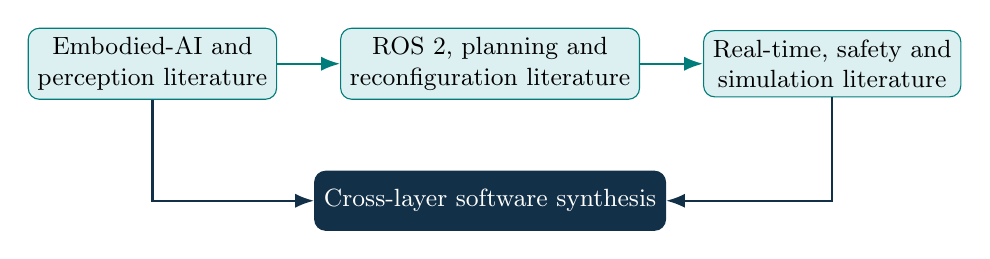
\begin{tikzpicture}[node distance=0.58cm and 0.8cm,every node/.style={font=\small,align=center},box/.style={draw=teal,fill=sky,rounded corners=4pt,minimum width=2.95cm,minimum height=0.75cm}]
\node[box] (ai) {Embodied-AI and\\ perception literature};
\node[box,right=of ai] (ros) {ROS~2, planning and\\ reconfiguration literature};
\node[box,right=of ros] (rt) {Real-time, safety and\\ simulation literature};
\node[draw=navy,fill=navy,text=white,rounded corners=4pt,minimum width=3.4cm,minimum height=0.75cm,below=0.9cm of ros] (synth) {Cross-layer software synthesis};
\draw[-{Latex[length=2.4mm]},thick,teal] (ai)--(ros);
\draw[-{Latex[length=2.4mm]},thick,teal] (ros)--(rt);
\draw[-{Latex[length=2.4mm]},thick,navy] (ai.south)|-(synth.west);
\draw[-{Latex[length=2.4mm]},thick,navy] (rt.south)|-(synth.east);
\end{tikzpicture}
\caption{Review methodology: layers are analysed separately and then reconciled through their execution and safety interfaces.}
\label{fig:method}
\end{figure}

\section{Software taxonomy and execution model}
\subsection{Multi-rate stack}
The literature consistently motivates a decoupled multi-rate pipeline. Cognitive services interpret intent and scene state; task services select recoverable skills; planning and integration services generate state-consistent trajectories; and local control executes only bounded commands. Table~\ref{tab:rates} formalises the taxonomy.

\begin{table}[ht]
\centering\small
\caption{Multi-rate software taxonomy for semi-humanoid mobile manipulators.}\label{tab:rates}
\begin{tabularx}{\textwidth}{@{}lrlY@{}}
\toprule
Layer & Indicative rate & Compute domain & Representative functions \\
\midrule
Cognition and perception & 5--10Hz & Edge GPU & OpenVLA/OpenVLA-OFT, panorama-aware VLA, JEPA-WAM, YOLOv11, SAM, speech-to-text, semantic 3D grounding \\
Task and planning & 30--100Hz & Host CPU/GPU & BehaviorTree.CPP, Nav2, MoveIt~2, DMPs, whole-body SDF/MPC, action graphs \\
Integration and communications & 100--500Hz & Linux host / middleware & \texttt{ros2\_control}, joint-state/control interfaces, DDS or \texttt{rmw\_zenoh}, iG-LIO, WMS/IoT and lifecycle management \\
Real-time and safety & 1kHz & MCU/RTOS or PREEMPT\_RT & FOC, joint/impedance loops, deadline monitor, tactile-force veto, E-stop and fieldbus services \\
Simulation and operations & asynchronous & Workstation/cloud/edge & OpenUSD assets, Isaac Lab, event-camera simulation, training, containers, OTA and telemetry \\
\bottomrule
\end{tabularx}
\evidence{Rates are architecture targets derived from the reviewed literature; deployment must establish measured WCET, jitter and end-to-end latency.}
\end{table}

\begin{figure}[ht]
\centering
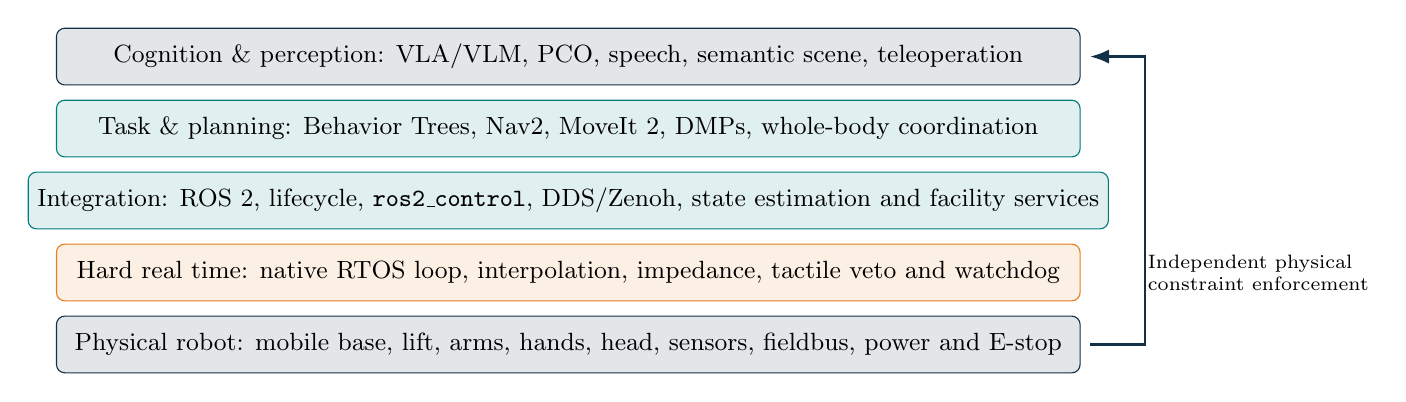
\begin{tikzpicture}[every node/.style={font=\small,align=center},layer/.style={draw=#1,fill=#1!12,rounded corners=3pt,minimum width=13.0cm,minimum height=0.72cm}]
\node[layer=navy] (cog) {Cognition \& perception: VLA/VLM, PCO, speech, semantic scene, teleoperation};
\node[layer=teal,below=0.18cm of cog] (task) {Task \& planning: Behavior Trees, Nav2, MoveIt~2, DMPs, whole-body coordination};
\node[layer=teal,below=0.18cm of task] (mid) {Integration: ROS~2, lifecycle, \texttt{ros2\_control}, DDS/Zenoh, state estimation and facility services};
\node[layer=orange,below=0.18cm of mid] (safe) {Hard real time: native RTOS loop, interpolation, impedance, tactile veto and watchdog};
\node[layer=navy,below=0.18cm of safe] (plant) {Physical robot: mobile base, lift, arms, hands, head, sensors, fieldbus, power and E-stop};
\draw[-{Latex[length=2.4mm]},thick,navy] ($(plant.east)+(0.12,0)$)--++(0.7,0)|-($(cog.east)+(0.12,0)$);
\node[right=0.73cm of safe,font=\scriptsize,align=left] {Independent physical\\ constraint enforcement};
\end{tikzpicture}
\caption{Reference architecture. The orange layer is the non-bypassable boundary between high-level software and physical actuation.}
\label{fig:stack}
\end{figure}

\section{Cognition, perception and action representation}
\subsection{Vision-language-action models and world models}
OpenVLA maps image and language inputs to 7-DoF action deltas and is reported to combine a 7B Llama~2 backbone with DINOv2 and SigLIP, pretrained on 970k Open X-Embodiment episodes. OpenVLA-OFT is reported to deliver 26$\times$ inference acceleration for edge fine-tuning.\cite{openvla,oft} Panorama-aware VLA extends this premise to dynamic mobile viewpoints; JEPA-WAM predicts stage-level visual outcomes for multi-step manipulation; and semantic 3D Gaussian Splatting grounds open-vocabulary language targets in 3D.\cite{pano,jepa,gaussian}

These methods are valuable action-proposal generators, not direct motor controllers. A formally useful interface represents an AI output as $(g,\Delta\mathbf{x},\Sigma,c)$: symbolic goal $g$, candidate Cartesian delta $\Delta\mathbf{x}$, uncertainty $\Sigma$, and confidence $c$. The autonomy system accepts only a projection into a verified feasible set:
\begin{equation}
\mathbf{x}_{\mathrm{ref}}=\Pi_{\mathcal{F}(\mathbf{q},\mathcal{E},\mathcal{S})}\!\left(\mathbf{x}+\Delta\mathbf{x}\right),
\end{equation}
where $\mathcal{F}$ includes kinematic, collision, payload, speed-zone, environment and safety-state constraints.

\subsection{Perception--cognition--operation and interaction}
The PCO framework provides a useful decomposition between perceptual estimation, semantic reasoning and motion operation.\cite{pco} In a semi-humanoid system, this accommodates RGB-D/LiDAR odometry, object detection/segmentation, language parsing, head orientation and human-facing feedback without collapsing all decisions into one learned policy. The perception layer should emit timestamped state estimates with frame IDs, confidence and freshness; downstream skills can reject stale or ambiguous evidence.

\section{Task autonomy, navigation and whole-body planning}
\subsection{Behavior Trees, DMPs and skill graphs}
Behavior Trees have a well-established role in modular reactivity and fault recovery relative to monolithic state machines.\cite{iovino} DMPs provide compact trajectory representations that can be adapted under perturbation.\cite{saveriano} RoboReact adds a reported route from egocentric demonstrations to executable ROS~2 action graphs.\cite{roboreact} Together, these methods support a layered task representation: Behavior Trees select and recover skills; DMPs/trajectory generators parameterise motion; and planners validate execution against current geometry.

\subsection{Nav2, MoveIt~2 and base--arm coupling}
Nav2 provides SLAM/localisation, route generation, costmaps and local planning such as DWB and MPPI. MoveIt~2 provides collision-aware inverse kinematics and trajectory planning for dual 6--7 DoF arms. The mobile base can be represented as a virtual $(x,y,\theta)$ joint in an SRDF/whole-body model. The central challenge is coordination: independent Nav2 and MoveIt execution can yield stop-then-move behaviour. Kinematically coupled SDF/MPC approaches aim to co-optimise base velocity and arm limits for payload-aware mobile manipulation.\cite{liwb,bonci}

\begin{figure}[ht]
\centering
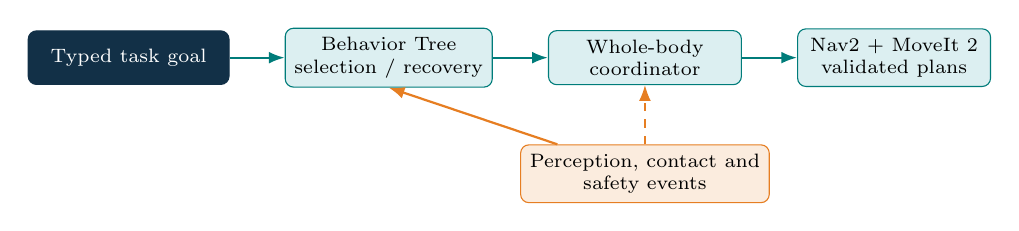
\begin{tikzpicture}[node distance=0.55cm and 0.7cm,every node/.style={font=\scriptsize,align=center},box/.style={draw=teal,fill=sky,rounded corners=3pt,minimum width=2.45cm,minimum height=0.68cm}]
\node[draw=navy,fill=navy,text=white,rounded corners=3pt,minimum width=2.55cm,minimum height=0.68cm] (goal) {Typed task goal};
\node[box,right=of goal] (bt) {Behavior Tree\\ selection / recovery};
\node[box,right=of bt] (coord) {Whole-body\\ coordinator};
\node[box,right=of coord] (plan) {Nav2 + MoveIt~2\\ validated plans};
\node[draw=orange,fill=orange!15,rounded corners=3pt,minimum width=2.6cm,minimum height=0.68cm,below=0.75cm of coord] (events) {Perception, contact and\\ safety events};
\draw[-{Latex[length=2mm]},thick,teal] (goal)--(bt);
\draw[-{Latex[length=2mm]},thick,teal] (bt)--(coord);
\draw[-{Latex[length=2mm]},thick,teal] (coord)--(plan);
\draw[-{Latex[length=2mm]},thick,orange] (events)--(bt.south);
\draw[-{Latex[length=2mm]},dashed,orange] (events)--(coord.south);
\end{tikzpicture}
\caption{Recoverable skill execution. The task layer receives asynchronous events and may re-plan, degrade or request assistance.}
\label{fig:skills}
\end{figure}

\section{Middleware, reconfiguration and robot integration}
ROS~2 supplies modular transport, discovery and lifecycle semantics for the software ecosystem. The \texttt{ros2\_control} abstraction standardises hardware interfaces, joint-state broadcasting and effort/position command distribution across heterogeneous VESC, ODrive and servo-drive actuators. Zenoh/\texttt{rmw\_zenoh} is presented as an alternative for local zero-copy shared-memory communication and efficient wireless publish/subscribe, whereas DDS remains an established ROS~2 default. Dynamic reconfiguration and lifecycle management address controlled node replacement and recovery without whole-system reboot.\cite{peldszus}

QoS must distinguish data freshness from delivery certainty: RGB-D/point-cloud paths favour bounded best-effort delivery; joint state, action result, configuration and safety state require reliable, deadline-aware contracts. Neither DDS nor Zenoh replaces the hardware safety path. iG-LIO and autonomous pallet picking provide examples of ROS~2 localisation and object-alignment integration, while WMS/IoT telemetry and QML/operator interfaces expose the facility-facing side of the stack.\cite{iglio,mokk}

\section{Real-time firmware, impedance and safety}
\subsection{Native control versus middleware callbacks}
Hard real-time loops should run in native FreeRTOS/Zephyr or bare-metal MCU tasks, decoupled from micro-ROS callbacks. The micro-ROS budget-based executor is relevant for command and telemetry scheduling, but XRCE-DDS serialization and callback scheduling must not determine a 1kHz motor deadline.\cite{micro} A priority structure places E-stop/deadline/overcurrent handling above servo control; servo and contact regulation above fieldbus processing; and fieldbus processing above telemetry and parameter updates.

\subsection{Impedance, tactile sensing and force veto}
VIDP is reported as a diffusion-policy approach for compliant, variable-impedance manipulation from diverse demonstrations.\cite{vidp} Conformal EIT touch skin provides a candidate geometry-scalable whole-body collision-sensing modality.\cite{eit} At the actuator boundary, the local controller uses a bounded impedance law,
\begin{equation}
\mathbf{F}_{\mathrm{cmd}}=\mathbf{K}(\mathbf{x}_d-\mathbf{x})+\mathbf{D}(\dot{\mathbf{x}}_d-\dot{\mathbf{x}}), \qquad
\tau_{\mathrm{cmd}}=K_p(q_d-q)+K_d(\dot q_d-\dot q)+\tau_{\mathrm{ff}},
\end{equation}
and independently saturates force, torque, velocity, acceleration and power. A tactile/force veto must transition the system into an explicit safe hold, compliant retreat or latched fault state; the cited 25N value is a proposed configuration point, not a universal safety threshold.

\begin{figure}[ht]
\centering
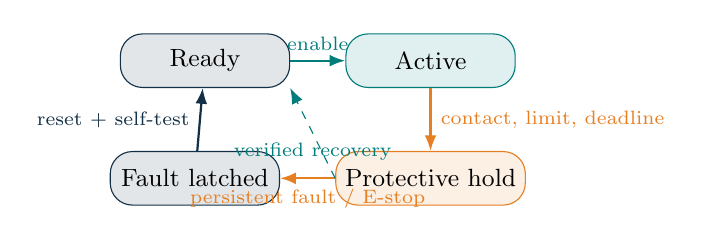
\begin{tikzpicture}[node distance=0.65cm and 0.7cm,every node/.style={font=\small,align=center},state/.style={draw=#1,fill=#1!12,rounded corners=8pt,minimum width=2.15cm,minimum height=0.68cm}]
\node[state=navy] (ready) {Ready};
\node[state=teal,right=of ready] (run) {Active};
\node[state=orange,below=0.8cm of run] (hold) {Protective hold};
\node[state=navy,left=of hold] (fault) {Fault latched};
\draw[-{Latex[length=2mm]},thick,teal] (ready)--node[above,font=\scriptsize]{enable} (run);
\draw[-{Latex[length=2mm]},thick,orange] (run)--node[right,font=\scriptsize]{contact, limit, deadline} (hold);
\draw[-{Latex[length=2mm]},thick,orange] (hold)--node[below,font=\scriptsize]{persistent fault / E-stop} (fault);
\draw[-{Latex[length=2mm]},dashed,teal] (hold.west)--node[below,font=\scriptsize]{verified recovery} (ready.south east);
\draw[-{Latex[length=2mm]},thick,navy] (fault)--node[left,font=\scriptsize]{reset + self-test} (ready);
\end{tikzpicture}
\caption{Safety state model for software-controlled execution. Hardware E-stop and power isolation remain independent protective measures.}
\label{fig:safety}
\end{figure}

\section{Digital twins, simulation and deployment}
OpenUSD provides a scene and asset representation for Isaac Sim/Isaac Lab, procedural environment generation and sensor simulation. EsaacSim extends Isaac Sim with event-camera and dynamic sensor models for visual-servoing studies.\cite{isaaclab,esaac} Digital-twin literature for human--robot collaboration motivates real-time synchronisation, collision-aware evaluation and operator-aware simulation.\cite{dtwin}

The software lifecycle should promote a capability through model-in-the-loop, SIL, vHIL, supervised hardware and bounded field deployment. Domain randomisation should include lighting, textures, sensor noise/latency, friction, payloads, wheel slip and contact conditions. Containerised deployment closes the remaining gap: build immutable images for VLA/perception, Nav2, MoveIt~2 and \texttt{ros2\_control}, then promote signed releases through simulation, bench, canary and fleet stages with telemetry and rollback.

\begin{figure}[ht]
\centering
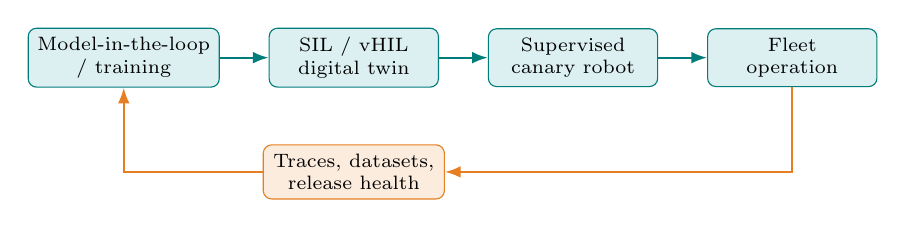
\begin{tikzpicture}[node distance=0.47cm and 0.62cm,every node/.style={font=\scriptsize,align=center},box/.style={draw=teal,fill=sky,rounded corners=3pt,minimum width=2.15cm,minimum height=0.65cm}]
\node[box] (model) {Model-in-the-loop\\ / training};
\node[box,right=of model] (sil) {SIL / vHIL\\ digital twin};
\node[box,right=of sil] (canary) {Supervised\\ canary robot};
\node[box,right=of canary] (fleet) {Fleet\\ operation};
\node[draw=orange,fill=orange!15,rounded corners=3pt,minimum width=2.3cm,minimum height=0.65cm,below=0.72cm of sil] (observe) {Traces, datasets,\\ release health};
\draw[-{Latex[length=2mm]},thick,teal] (model)--(sil);
\draw[-{Latex[length=2mm]},thick,teal] (sil)--(canary);
\draw[-{Latex[length=2mm]},thick,teal] (canary)--(fleet);
\draw[-{Latex[length=2mm]},thick,orange] (fleet.south)|-(observe.east);
\draw[-{Latex[length=2mm]},thick,orange] (observe.west)-|(model.south);
\end{tikzpicture}
\caption{Sim-to-real and release lifecycle. Observability and rollback gates transform deployment into a controlled experiment.}
\label{fig:lifecycle}
\end{figure}

\section{Open problems and research agenda}
\begin{longtable}{@{}p{0.26\textwidth}p{0.32\textwidth}p{0.32\textwidth}@{}}
\caption{Unified software research agenda.}\label{tab:gaps}\\
\toprule
Research gap & Failure mode & Required research artefact \\
\midrule
\endfirsthead
\toprule Research gap & Failure mode & Required research artefact \\
\midrule\endhead
VLA-to-control rate disparity & Raw 5--10Hz deltas yield discontinuous or unsafe execution & Trajectory interpolator plus variable-impedance filter; latency, smoothness and contact-safety benchmark \\
Base--arm kinematic coupling & Nav2 and MoveIt~2 create stop-then-move or dynamically awkward behaviour & Open whole-body coordinator; payload, clearance and throughput comparison against sequential planning \\
Bimanual BT recovery & Single-arm/navigation trees do not manage slip, blocked transport or handover failure & Reusable recovery-node library and benchmark with recovery success/time-to-recovery \\
Micro-ROS timing jitter & Callback-driven control violates hard timing budgets & Native RTOS control task with measured WCET/jitter; micro-ROS used only as asynchronous bridge \\
Cloud-to-edge reproducibility & Simulator/host dependency drift causes deployment breakages & Open container manifests, hardware configuration schema, signed OTA and rollback evaluation \\
Vision-only VLA contact blindness & Occlusion/unknown contact causes inappropriate action continuation & \texttt{ros2\_control}-integrated tactile/F/T/EIT veto with fault-injection evidence \\
\bottomrule
\end{longtable}

\section{Conclusion}
The literature establishes a robust vocabulary for semi-humanoid software: VLA and world models for semantic proposals; PCO for functional decomposition; Behavior Trees and DMPs for recoverable task execution; Nav2, MoveIt~2 and whole-body planning for mobile manipulation; ROS~2, \texttt{ros2\_control} and Zenoh/DDS for integration; native MCU firmware for hard timing; and OpenUSD digital twins for validation. The outstanding research contribution is the verified connection of these layers. Future systems should demonstrate, rather than assume, that high-level intelligence is constrained by time-stamped plans, that middleware is isolated from servo deadlines, that tactile contact can veto vision-derived actions, and that releases transfer from simulation to fleets with traceable evidence.

\begin{thebibliography}{99}\small
\bibitem{openvla} M. J. Kim et al., ``OpenVLA: An Open-Source Vision-Language-Action Model,'' arXiv:2406.09246, 2024. \url{https://arxiv.org/abs/2406.09246}.
\bibitem{oft} M. J. Kim et al., ``Fine-Tuning Vision-Language-Action Models: Optimizing Speed and Success,'' arXiv:2502.19645, 2025. \url{https://arxiv.org/abs/2502.19645}.
\bibitem{pano} D. Yang, H. Chen, and X. Chen, ``Learning Panorama-Aware VLA for Mobile Manipulation with Whole-Body Teleoperation,'' arXiv:2608.02257, 2026. \url{https://arxiv.org/abs/2608.02257}.
\bibitem{jepa} X. Liu, Y. Yang, and X. Wang, ``JEPA-WAM,'' arXiv:2608.10780, 2026. \url{https://arxiv.org/abs/2608.10780}.
\bibitem{gaussian} H. Ou, D. Song, and Y. Wang, ``Embodied Multimodal Grounding via Semantic 3D Gaussian Splatting,'' arXiv:2608.10756, 2026. \url{https://arxiv.org/abs/2608.10756}.
\bibitem{pco} M. V. L. Carvalho, L. R. Yoshioka, and J. F. Justo, ``The Perception--Cognition--Operation Approach,'' 2026. DOI: \url{https://doi.org/10.20944/preprints202603.0528.v1}.
\bibitem{iovino} M. Iovino et al., ``A Survey of Behavior Trees in Robotics and AI,'' \emph{Robotics and Autonomous Systems}, 2022. DOI: \url{https://doi.org/10.1016/j.robot.2022.104096}.
\bibitem{saveriano} M. Saveriano, F. J. Abu-Dakka, and A. Kramberger, ``Dynamic Movement Primitives in Robotics,'' \emph{IJRR}, 2023. DOI: \url{https://doi.org/10.1177/02783649231201196}.
\bibitem{roboreact} T. He et al., ``RoboReact,'' arXiv:2608.03387, 2026. \url{https://arxiv.org/abs/2608.03387}.
\bibitem{liwb} Y. Li, L. Yin, and T. Zhang, ``Kinematically-Coupled SVSDF Whole-Body Planning,'' arXiv:2608.07005, 2026. \url{https://arxiv.org/abs/2608.07005}.
\bibitem{bonci} A. Bonci, F. Gaudeni, and M. Giannini, ``ROS2-Based Frameworks for Increasing Robot Autonomy,'' \emph{Applied Sciences}, 2023. DOI: \url{https://doi.org/10.3390/app132312796}.
\bibitem{peldszus} S. Peldszus, D. Brugali, and D. Strüber, ``Software Reconfiguration in Robotics,'' arXiv:2310.01039, 2023. \url{https://arxiv.org/abs/2310.01039}.
\bibitem{iglio} A. E. Carvalho, D. Portugal, and P. Peixoto, ``A Numerically-Robust ROS~2 Port of iG-LIO,'' arXiv:2607.09947, 2026. \url{https://arxiv.org/abs/2607.09947}.
\bibitem{mokk} T. Mökkönen, ``Autonomous Pallet Picking Using ROS2,'' Tampere University, 2024. \url{https://trepo.tuni.fi/handle/10024/154752}.
\bibitem{micro} N. Stoufs et al., ``Budget-Based Real-Time Executor for Micro-ROS,'' arXiv:2105.05590, 2021. \url{https://arxiv.org/abs/2105.05590}.
\bibitem{vidp} H. Khalil, N. Fernandes, and T. M. Kwok, ``VIDP: Variable Impedance Diffusion Policy,'' arXiv:2608.06210, 2026. \url{https://arxiv.org/abs/2608.06210}.
\bibitem{eit} H. Chen, C. Kohlbrenner, and J. Kubik, ``Geometry-Scalable Whole-Body Touch for Humanoids,'' arXiv:2608.02080, 2026. \url{https://arxiv.org/abs/2608.02080}.
\bibitem{isaaclab} M. Mittal et al., ``Isaac Lab,'' arXiv:2403.07257, 2024. \url{https://arxiv.org/abs/2403.07257}.
\bibitem{esaac} I. Bugueno-Cordova et al., ``EsaacSim,'' arXiv:2608.08522, 2026. \url{https://arxiv.org/abs/2608.08522}.
\bibitem{dtwin} A. K. Ramasubramanian, R. Mathew, and M. Kelly, ``Digital Twin for Human--Robot Collaboration in Manufacturing,'' \emph{Applied Sciences}, 2022. DOI: \url{https://doi.org/10.3390/app12104811}.
\end{thebibliography}
\end{document}
